% !TeX root = wj-tree-design.tex
% 在项目根运行；独立预览，不接入正式讲义。
\documentclass[UTF8,fontset=none,11pt]{ctexart}
\usepackage[a4paper,margin=19mm]{geometry}
\usepackage{amsmath,amssymb,tikz}
\usetikzlibrary{calc,arrows.meta}
% 项目统一中文字体：避免依赖某台电脑上的 STSong/STHeiti 等系统字体。
\setCJKmainfont{SourceHanSerifCN-Regular.ttf}[
    Path = fonts/,
    BoldFont = SourceHanSerifCN-Bold.ttf,
    ItalicFont = AR-PL-KaitiM-GB.ttf,
    BoldItalicFont = AR-PL-KaitiM-GB.ttf,
    BoldItalicFeatures = {FakeBold = 2},
]
\setCJKsansfont{SourceHanSansCN-Regular.ttf}[
    Path = fonts/,
    BoldFont = SourceHanSansCN-Bold.ttf,
]
\setCJKmonofont{SourceHanSansCN-Regular.ttf}[
    Path = fonts/,
]

% fontset=none 时 CTeX 不创建这些常用字体族命令，显式补齐。
\setCJKfamilyfont{zhsong}{SourceHanSerifCN-Regular.ttf}[Path = fonts/]
\setCJKfamilyfont{zhhei}{SourceHanSansCN-Bold.ttf}[Path = fonts/]
\setCJKfamilyfont{zhkai}{AR-PL-KaitiM-GB.ttf}[Path = fonts/]
\setCJKfamilyfont{zhfs}{SourceHanSerifCN-Regular.ttf}[Path = fonts/]
\providecommand{\songti}{\CJKfamily{zhsong}}
\providecommand{\heiti}{\CJKfamily{zhhei}}
\providecommand{\kaishu}{\CJKfamily{zhkai}}
\providecommand{\fangsong}{\CJKfamily{zhfs}}

% 王江讲义树图候选样式；由正式入口加载 tikz、calc、arrows.meta 后接入。
% 单期接口兼容既有 \WJEventTree；接入时替换旧定义，勿重复定义。
\makeatletter
\newif\ifWJ@tree@stem
\pgfkeys{
  /WJ tree/.is family,
  /WJ tree/left/.initial={},
  /WJ tree/stem/.code=\WJ@tree@stemtrue,
  /WJ tree/row sep/.initial=1.7em,
}
\NewDocumentCommand{\WJEventTree}{O{} m}{%
  \begingroup
  \WJ@tree@stemfalse
  \pgfqkeys{/WJ tree}{#1}%
  \begin{tikzpicture}[x=1em,y=1em,baseline=(current bounding box.center)]
    \def\WJ@n{0}%
    \foreach \WJ@lab [count=\WJ@i] in {#2} {\xdef\WJ@n{\WJ@i}}%
    \pgfmathsetlengthmacro{\WJ@dy}{\pgfkeysvalueof{/WJ tree/row sep}}%
    \pgfmathsetlengthmacro{\WJ@ymax}{\WJ@dy*(\WJ@n-1)/2}%
    \draw[line width=.4pt,line cap=butt] (0,\WJ@ymax) -- (0,-\WJ@ymax);
    \foreach \WJ@lab [count=\WJ@i] in {#2} {%
      \pgfmathsetlengthmacro{\WJ@y}{\WJ@ymax-\WJ@dy*(\WJ@i-1)}%
      \draw[line width=.4pt,line cap=butt] (0,\WJ@y) -- (.7,\WJ@y);
      % mid west 将数学轴置于支线高度；不再使用 base west 和手工 yshift。
      \node[anchor=mid west,inner xsep=.28em,inner ysep=0pt]
        at (.7,\WJ@y) {$\WJ@lab$};
    }%
    \pgfkeysgetvalue{/WJ tree/left}\WJ@left
    \ifx\WJ@left\empty\else
      \WJ@tree@stemtrue
      \node[anchor=mid east,inner xsep=.22em,inner ysep=0pt]
        at (-.85,0) {\WJ@left};
    \fi
    \ifWJ@tree@stem
      \draw[line width=.4pt,line cap=butt] (-.85,0) -- (0,0);
    \fi
  \end{tikzpicture}%
  \endgroup
}
\makeatother

% 多期二叉树：节点为先、连线为后；不预设重合或路径展开结构。
% 参考 431《金融衍生品》具名节点和按时点分列的布局，本项目独立维护。
\tikzset{
  WJ binomial/.style={font=\small,baseline=(current bounding box.center)},
  WJ binomial compact/.style={WJ binomial,x=2.3cm,y=.78cm},
  WJ binomial node/.style={align=center,inner xsep=2pt,inner ysep=1pt,
    minimum width=7mm,minimum height=5mm,outer sep=1pt,
    execute at begin node={\setlength{\baselineskip}{10.5pt}}},
  WJ binomial edge/.style={-{Stealth[length=1.5mm,width=1mm]},line width=.45pt},
  WJ binomial time/.style={font=\small,anchor=north,inner sep=1pt},
}

\setlength{\parindent}{2em}
\pagestyle{plain}
\begin{document}
\begin{center}\Large 单期状态树与多期二叉树\end{center}
\section*{单期：当期节点与下一期状态支付}
左侧为当期值，右侧为下一期不同状态的结果。采用水平分叉，根节点和叶节点统一按数学轴对齐；状态数可扩展，分数标签可增大行距。
\begin{center}
\begin{tabular}{@{}c@{\hspace{2cm}}c@{}}
\WJEventTree[left={$e_1{:}100$}]{0,0}&
\WJEventTree[left={$e_2{:}0$}]{200,100,50}\\[1em]
两状态禀赋 & 三状态禀赋\\[2em]
\WJEventTree[left={$\tfrac12$},row sep=2em]{\tfrac32,\tfrac12}&
\WJEventTree[stem]{1,2,3}\\[1em]
分数节点 & 无当期值的支付向量
\end{tabular}
\end{center}
\vspace{1em}
\begin{center}
\WJEventTree[left={$S$}]{uS\text{，状态 }u\text{，概率 }\pi,
 dS\text{，状态 }d\text{，概率 }1-\pi}
\end{center}

\section*{适用边界}
单期树表达同一未来时点的多个状态，纵向位置用于排列状态。它可以放在正文、题目和解答中；既有状态顺序、数值和概率保持不变。水平支线只连接竖干与标签，不穿过数字，也不伸出首尾分叉。

\newpage
\section*{多期：按时点展开、按节点倒推}
每个时点为一列，列距为 $2.3$ cm；斜线连接节点边缘，数字位于节点内，双行文字采用紧凑行距。题目图只放给定数据；解答图需要时将股价置于上行、期权价值置于下行。本页价格与期权价值使用 431 两期算例作为排版示范。
\begin{center}
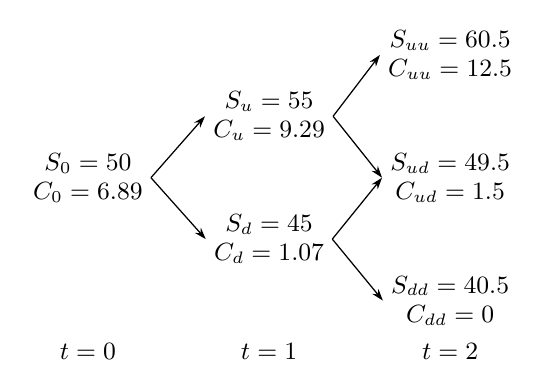
\begin{tikzpicture}[WJ binomial compact]
\node[WJ binomial node] (A) at (0,0) {$S_0=50$\\$C_0=6.89$};
\node[WJ binomial node] (B) at (1,1) {$S_u=55$\\$C_u=9.29$};
\node[WJ binomial node] (C) at (1,-1) {$S_d=45$\\$C_d=1.07$};
\node[WJ binomial node] (D) at (2,2) {$S_{uu}=60.5$\\$C_{uu}=12.5$};
\node[WJ binomial node] (E) at (2,0) {$S_{ud}=49.5$\\$C_{ud}=1.5$};
\node[WJ binomial node] (F) at (2,-2) {$S_{dd}=40.5$\\$C_{dd}=0$};
\foreach \a/\b in {A/B,A/C,B/D,B/E,C/E,C/F}
  \draw[WJ binomial edge] (\a.east) -- (\b.west);
\foreach \x/\t in {0/0,1/1,2/2}
  \node[WJ binomial time] at (\x,-2.65) {$t=\t$};
\end{tikzpicture}
\end{center}
只依赖当前股价的支付可以使用重合树；依赖历史路径的支付，应保留上涨后下跌与下跌后上涨两条路径。
\begin{center}
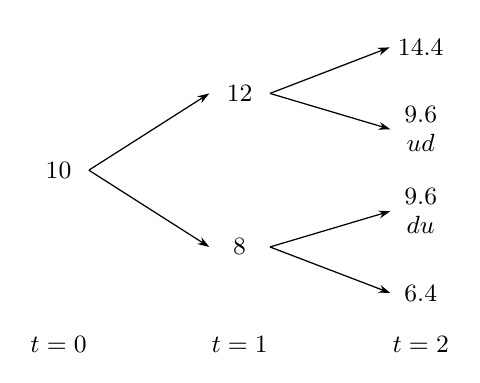
\begin{tikzpicture}[WJ binomial compact]
\node[WJ binomial node] (A) at (0,0) {$10$};
\node[WJ binomial node] (B) at (1,1.25) {$12$};
\node[WJ binomial node] (C) at (1,-1.25) {$8$};
\node[WJ binomial node] (D) at (2,2) {$14.4$};
\node[WJ binomial node] (E) at (2,.6667) {$9.6$\\$ud$};
\node[WJ binomial node] (F) at (2,-.6667) {$9.6$\\$du$};
\node[WJ binomial node] (G) at (2,-2) {$6.4$};
\foreach \a/\b in {A/B,A/C,B/D,B/E,C/F,C/G}
  \draw[WJ binomial edge] (\a.east) -- (\b.west);
\foreach \x/\t in {0/0,1/1,2/2}
  \node[WJ binomial time] at (\x,-2.65) {$t=\t$};
\end{tikzpicture}
\end{center}
保留路径的示例沿用王江练习的数据；重复的 $9.6$ 对应两条不同路径，不因数值相同而删除。
\end{document}
